\section{Topology Design Anti-Patterns}

This section and section \ref{algo} elaborate on the Anti-patterns and algorithmic analysis supported in OSTIA. All figures in these sections use a simple graph-like notation where nodes may be any topological element (e.g., Spouts or Bolts in Apache Storm terms) while edges are to be interpreted as directed data-flow connections.

\label{sec:anti-pattern}
This elaborates on the anti-patterns we elicited through self-ethnography. These anti-patterns are elaborated further within OSTIA to allow for their detection during streaming topology inference analysis.

\subsection{Multi-Anchoring}
In order to guarantee fault-tolerant stream processing, tuples processed by bolts needs to be anchored with the unique id of the bolt and be passed to multiple acknowledgers (or ``ackers" in short) in the topology. In this way, ackers can keep track of tuples in the topology.\\
%\emph{\bf TODO: what is the consequence of these anti-patterns? How does OSTIA detect?}
%\emph{\bf Multi-anchoring is not supported at the moment. Besides, I am not sure it is an anti-patter but rather a design decision}

%\begin{figure}[H]
%	\begin{center}
%		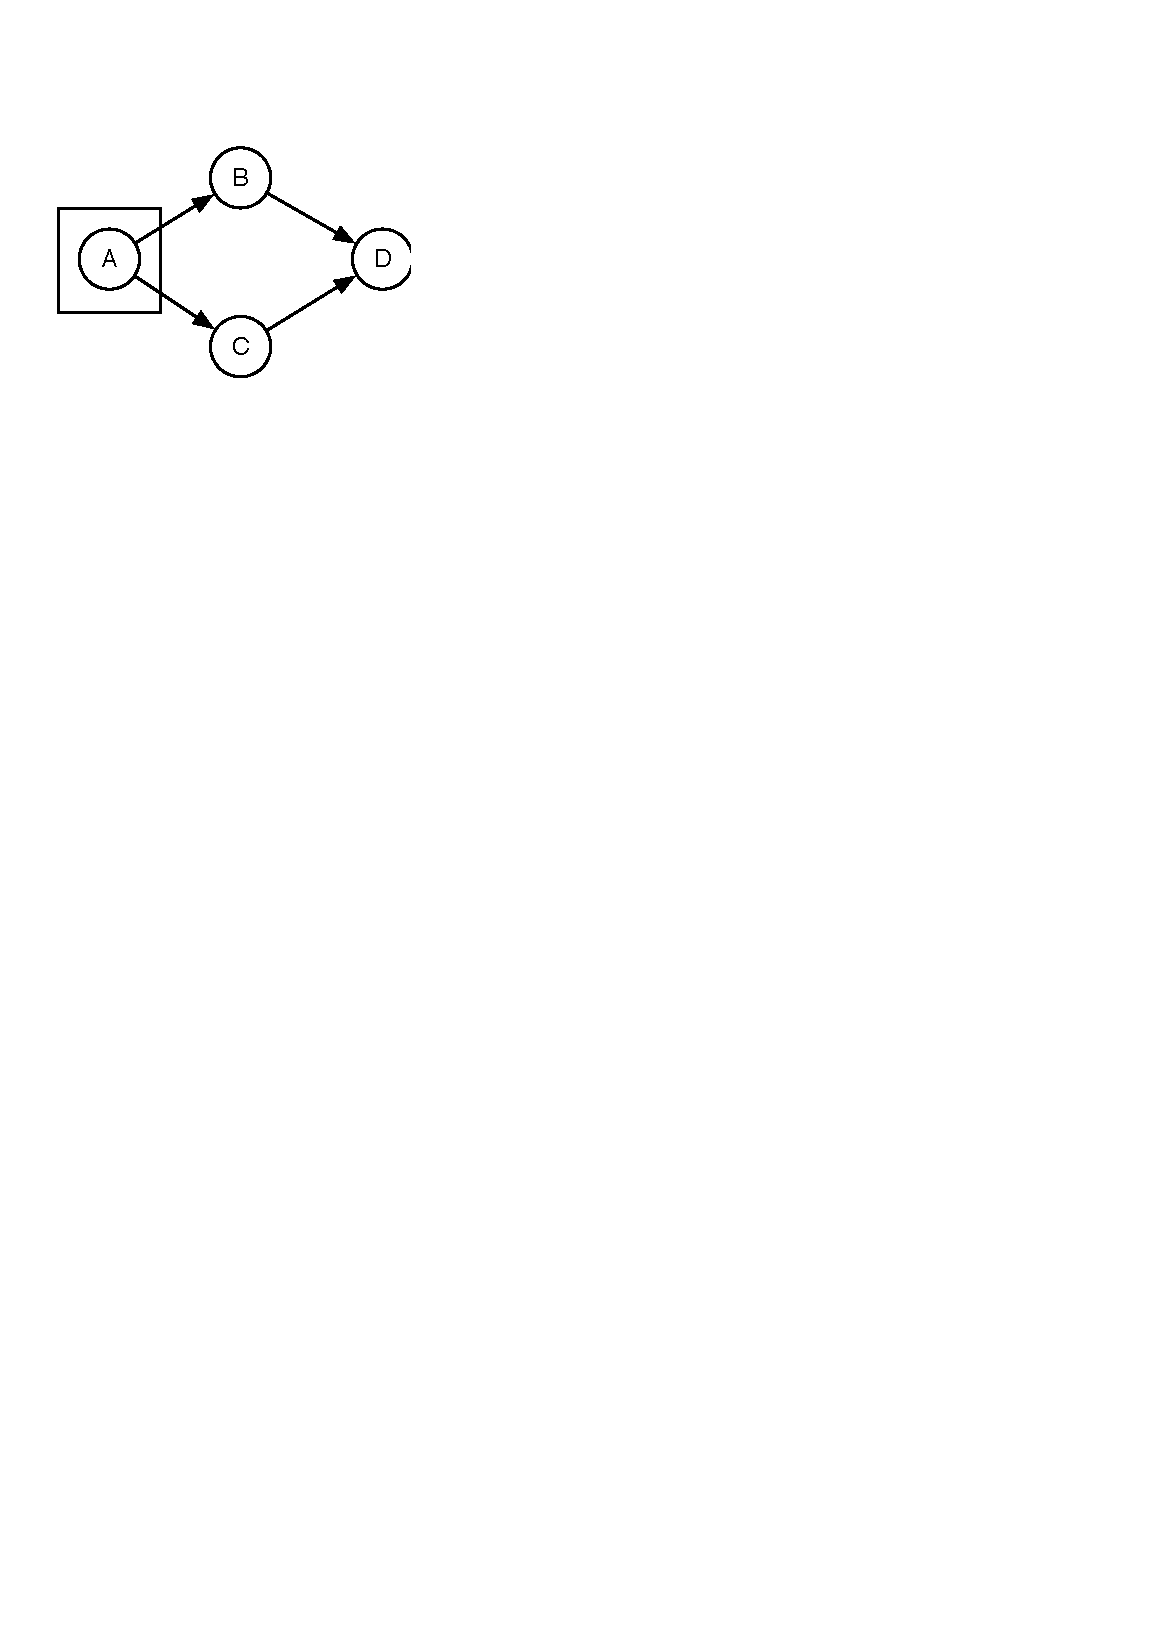
\includegraphics[width=2.5cm]{images/multi-anchoring}
%		\caption{Multi-anchoring.}
%		\label{fig:multi-anchoring}
%	\end{center}
%\end{figure}

\begin{figure}
\centering 
\subfigure[Multi-anchoring.]{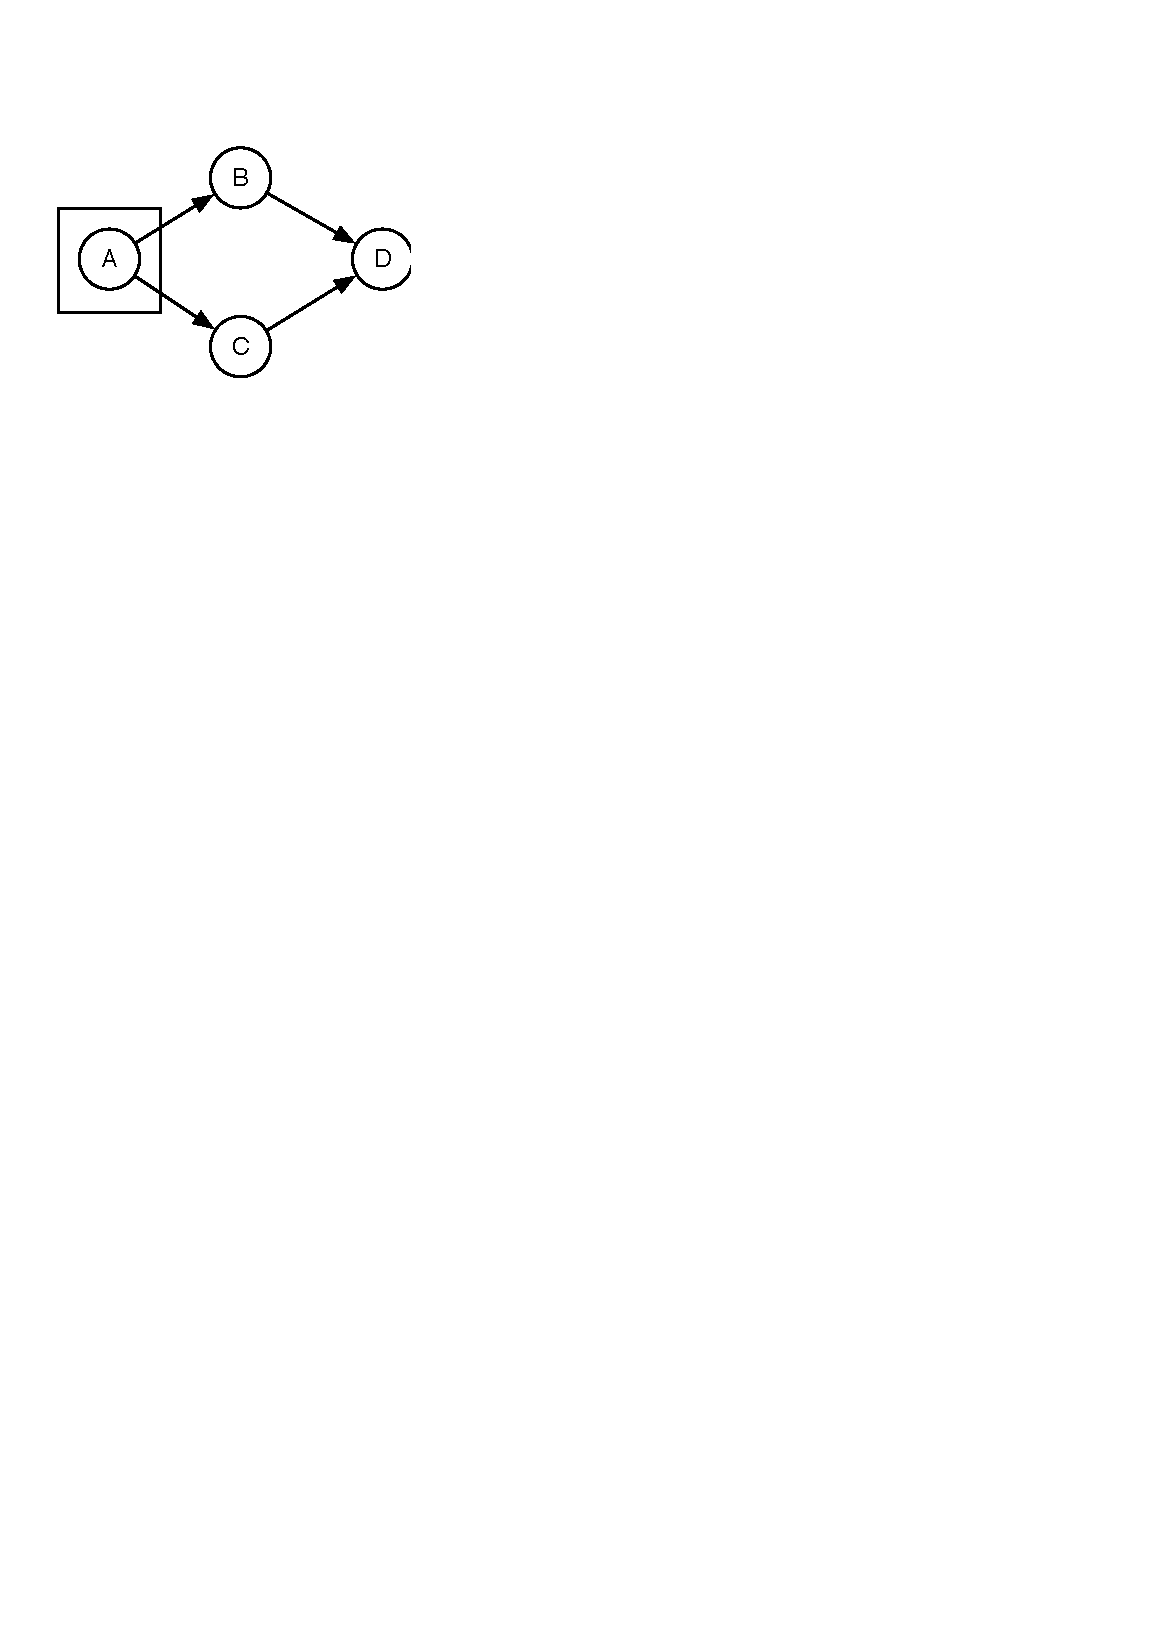
\includegraphics[width=2.5cm]{images/multi-anchoring}}\label{fig:multi-anchoring}
\hspace{1cm}
\subfigure[Cycle-in.]{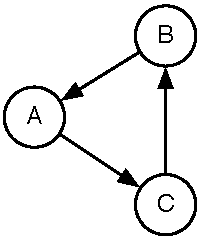
\includegraphics[width=2.0cm]{images/cycle}}\label{fig:cycle}
\end{figure}


\subsection{Cycle-in Topology}

Technically, it is possible to have cycle in Storm topologies. An infinite cycle of processing would create an infinite tuple tree and make it impossible for Storm to ever acknowledge spout emitted tuples. Therefore, cycles should be avoided or resulting tuple trees should be investigated additionally to make sure they terminate at some point and under a specified series of conditions. The anti-pattern itself may lead to infrastructure overloading and therefore increased costs.
%\emph{\bf A topology is already an infinite stream of tuple, the problem could be the overloading of some machines}
%\emph{\bf At the cycle-detection is not supported (even if it is easy to implement)}

%\begin{figure}[H]
%	\begin{center}
%		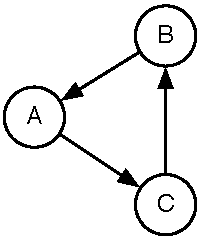
\includegraphics[width=2cm]{images/cycle}
%		\caption{Cycle-in Topology.}
%		\label{fig:cycle}
%	\end{center}
%\end{figure}

\subsection{Persistent Data}

This pattern covers the circumstance wherefore if two processing elements need to update a same entity in a storage, there should be a consistency mechanism in place. OSTIA offers limited support to this feature, which we plan to look into more carefully for future work. More details on this support are discussed in the approach limitations section (see Sec. \ref{lim}).
%\emph{\bf Ostia does not support this. BTW is this static analysis? if not, is it off-topic?}

\begin{figure}[H]
	\begin{center}
		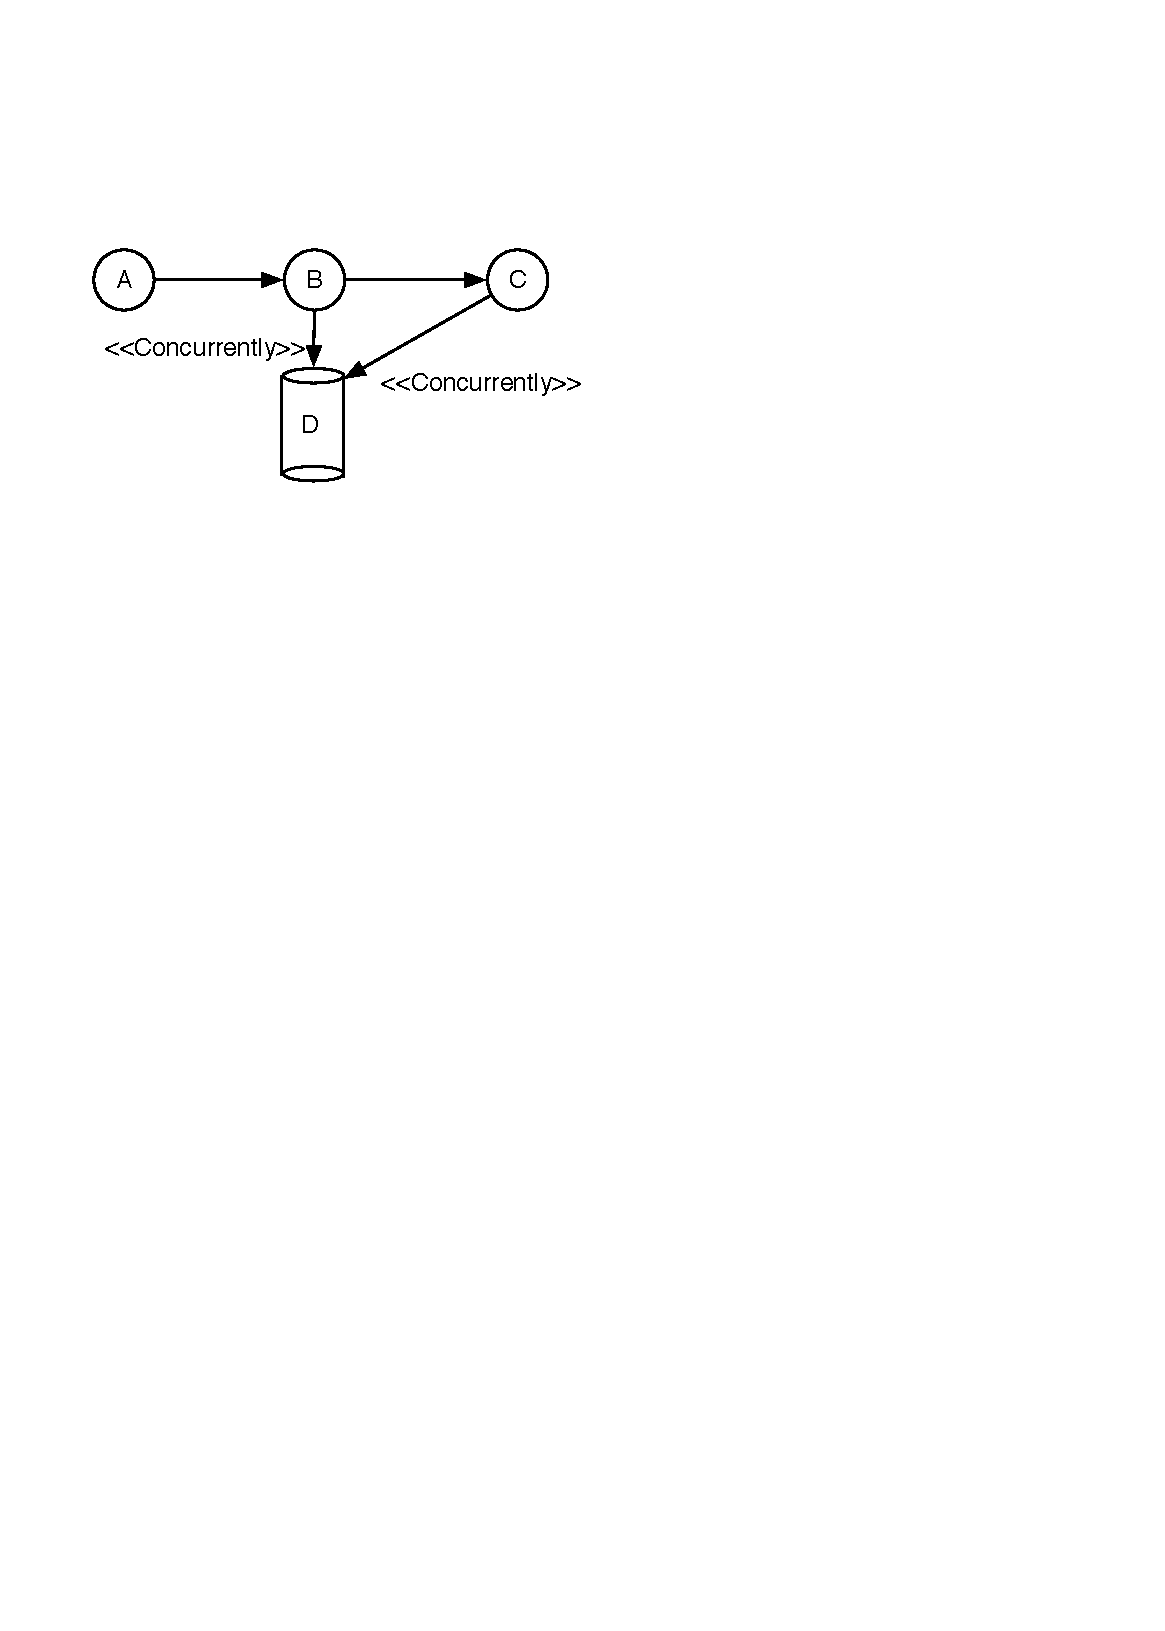
\includegraphics[width=4cm]{images/persistence}
		\caption{Concurrency management in case of Persistent Data circumstances.}
		\label{fig:persistence}
	\end{center}
\end{figure}


\subsection{Computation funnel}
A computational funnel emerges when there is not a path from data source (spout) to the bolts that sends out the tuples off the topology to another topology through a messaging framework or through a storage. This circumstance should be dealt with since it may compromise the availability of results under the desired performance restrictions.

\begin{figure}[H]
	\begin{center}
		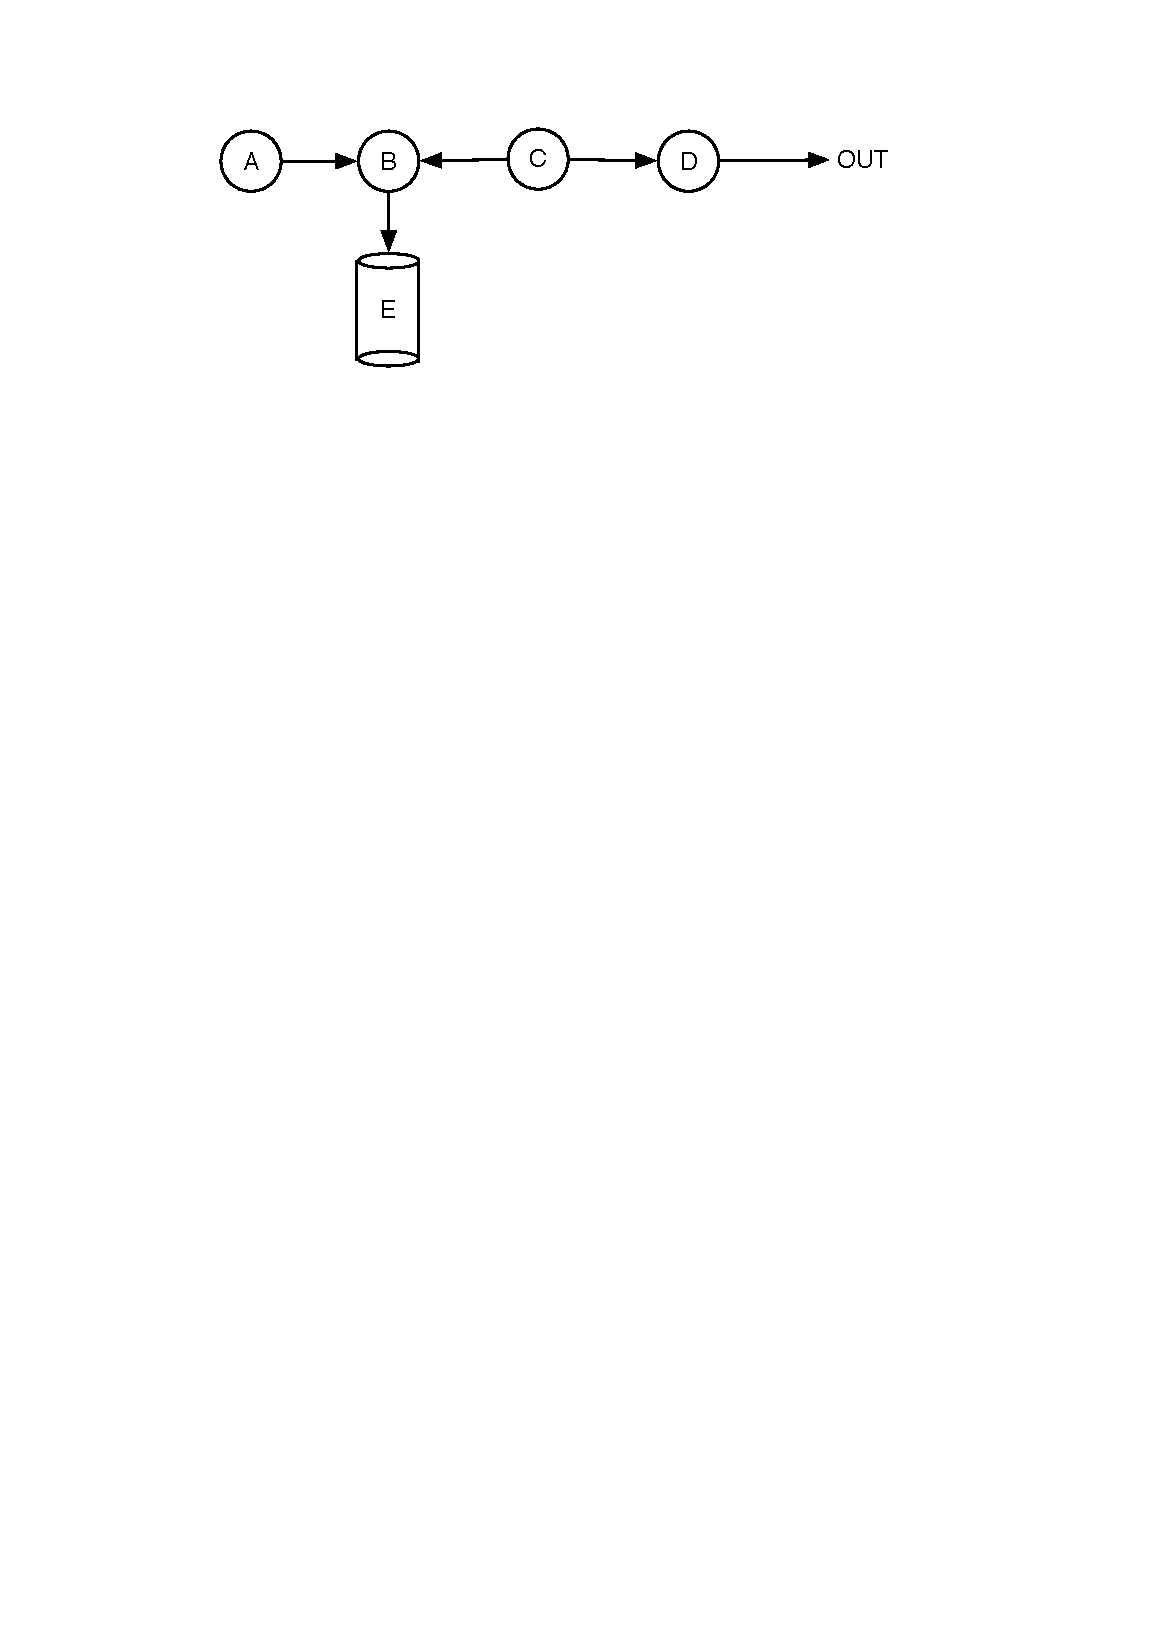
\includegraphics[width=5cm]{images/funnel}
		\caption{computation funnel.}
		\label{fig:funnel}
	\end{center}
\end{figure}

\section{Algorithmic Analysis on Stream Topologies}\label{algo}

\subsection{fan-in/fan-out}

For each element of the topology, fan-in is the number of incoming
streams. Conversely, fan-out is the number outgoing streams. In the case of
bolts, both in and out streams are internal to the topology. For Spouts,
incoming streams are the data sources of the topology (e.g., message brokers,
APIs, etc).

\begin{figure}[H]
	\begin{center}
		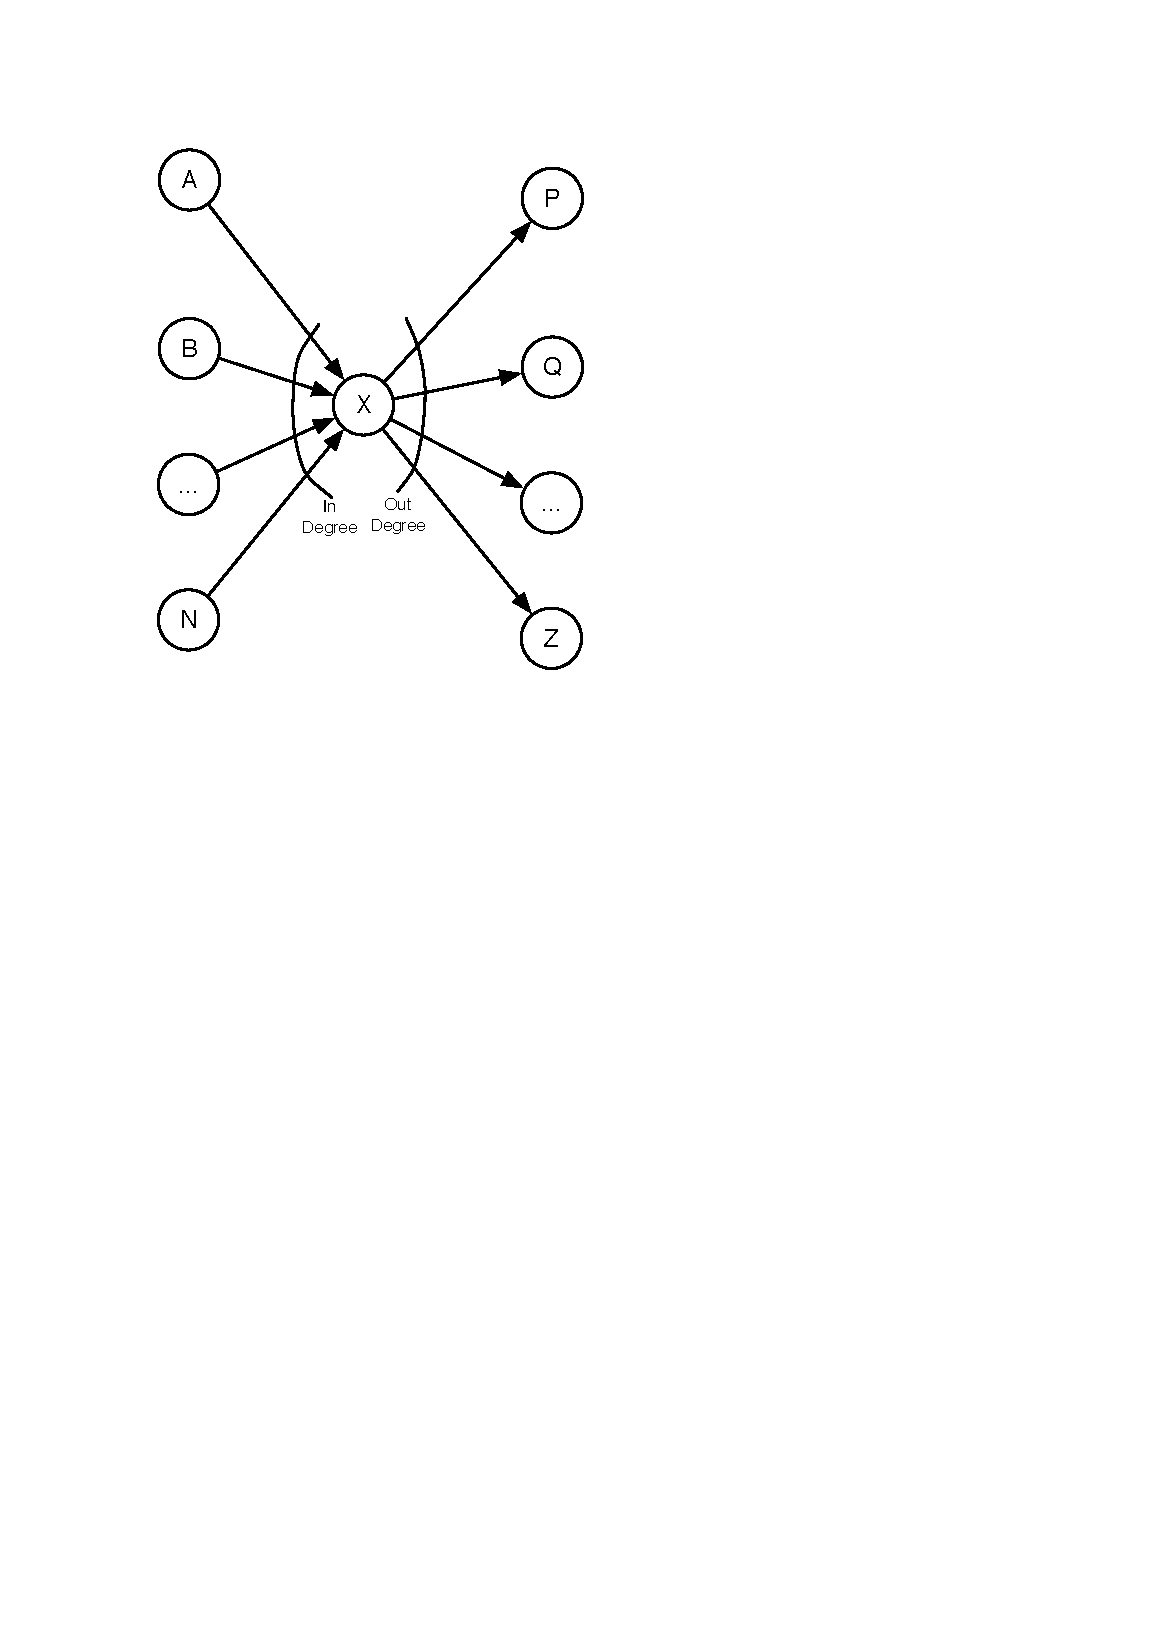
\includegraphics[width=3cm]{images/fan-in-out}
		\caption{Fan-in fan-out in Stream topologies.}
		\label{fig:fan}
	\end{center}
\end{figure}

This algorithmic manipulation allows to visualise instances where fan-in and fan-out numbers are differing.

\subsection{topology cascading}

By topology cascading, we mean connecting two different Storm topologies via a messaging framework (e.g., Apache Kafka). This circumstance, which is actually part of our evaluation and case-studies, may raise the complexity of the overarching topology to unacceptable levels and may require additional attention. OSTIA support for this feature is still limited, more details on this and similar limitations are discussed in Section \ref{lim}.
%\emph{\bf Ostia does not support this. I can't think of an easy way to implement it}

\begin{figure}[H]
	\begin{center}
		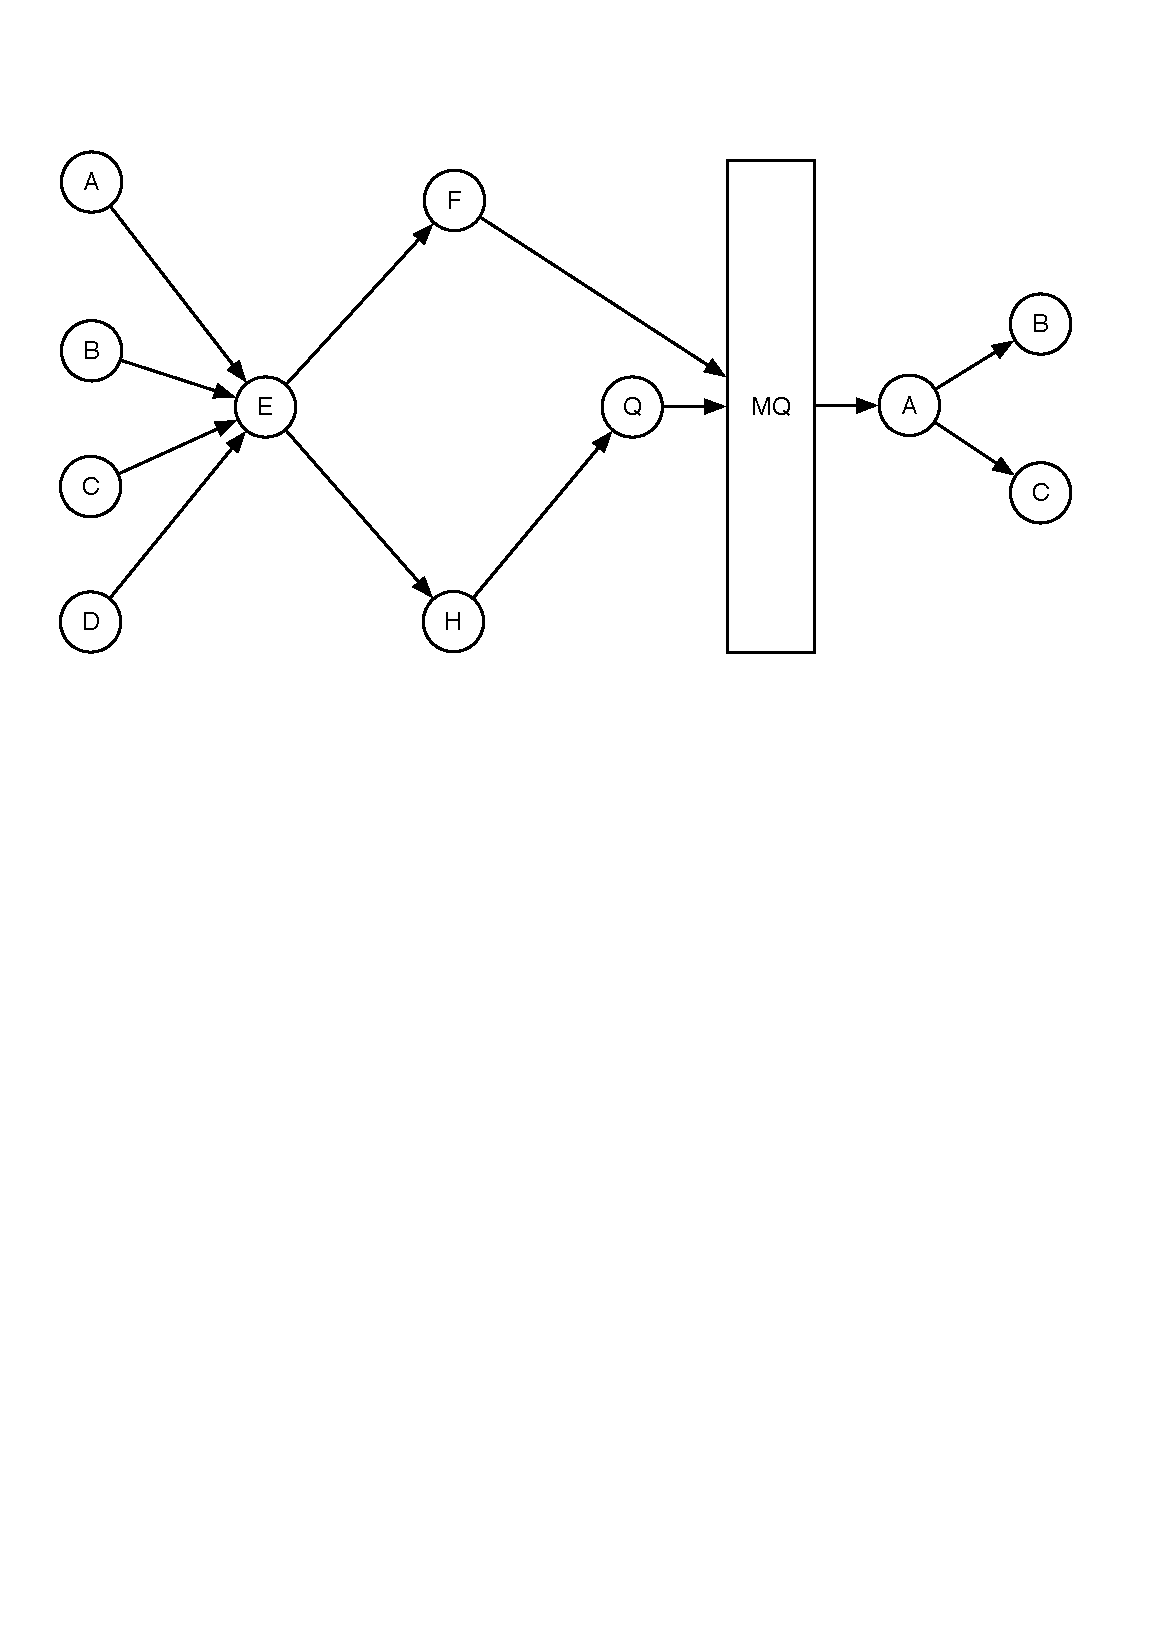
\includegraphics[width=6cm]{images/cascading}
		\caption{cascading.}
		\label{fig:cascading}
	\end{center}
\end{figure}

This algorithmic manipulation allows to combine multiple cascading topologies.

\subsection{Topology clustering}
Identifying the coupled processing elements and put the in a cluster in a way that elements in a cluster have high cohesion and less coupled with the elements in other clusters. Simple clustering or Social-Network Analysis mechanisms can be used to infer clusters. These clusters may require additional attention since they could turn out to become bottlenecks. Reasoning more deeply on clusters and their resolution may lead to establishing the Storm scheduling policy best-fitting with the application at hand.
%\emph{\bf Does it relates with Storm scheduling?}

\begin{figure}[H]
	\begin{center}
		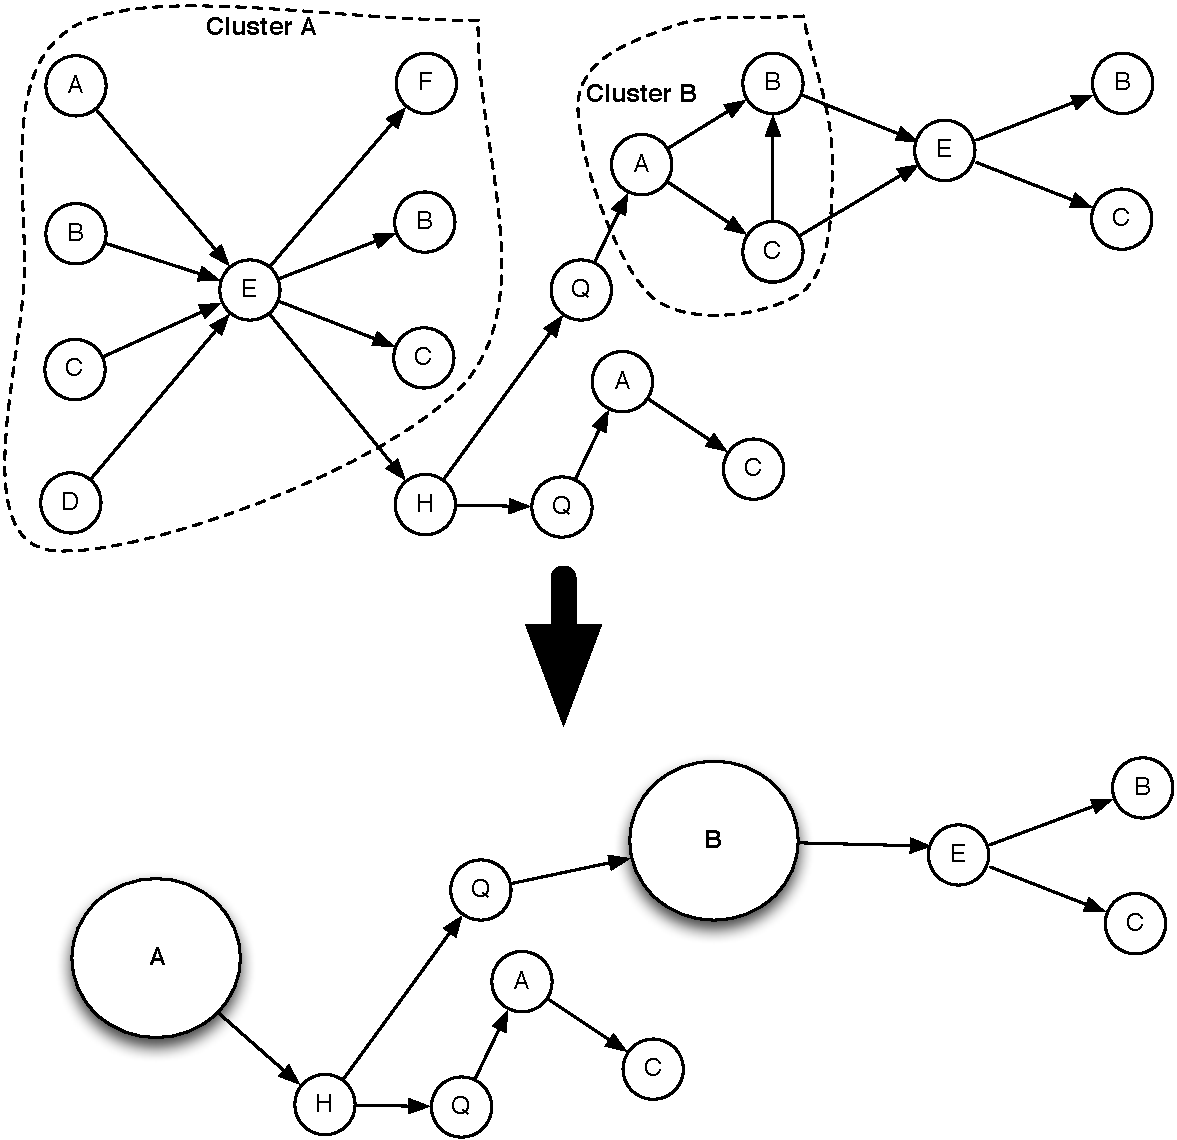
\includegraphics[width=5cm]{images/clustering}
		\caption{clustering.}
		\label{fig:clustering}
	\end{center}
\end{figure}

\subsection{Linearising a topology}

Sorting the processing elements in a topology in a way that topology looks more linear, visually. This step ensures that visual investigation and evaluation of the structural complexity of the topology is possible by direct observation. It is sometimes essential to provide such a visualisation to evaluate how to refactor the topology based on emerging needs.

\begin{figure}[H]
	\begin{center}
		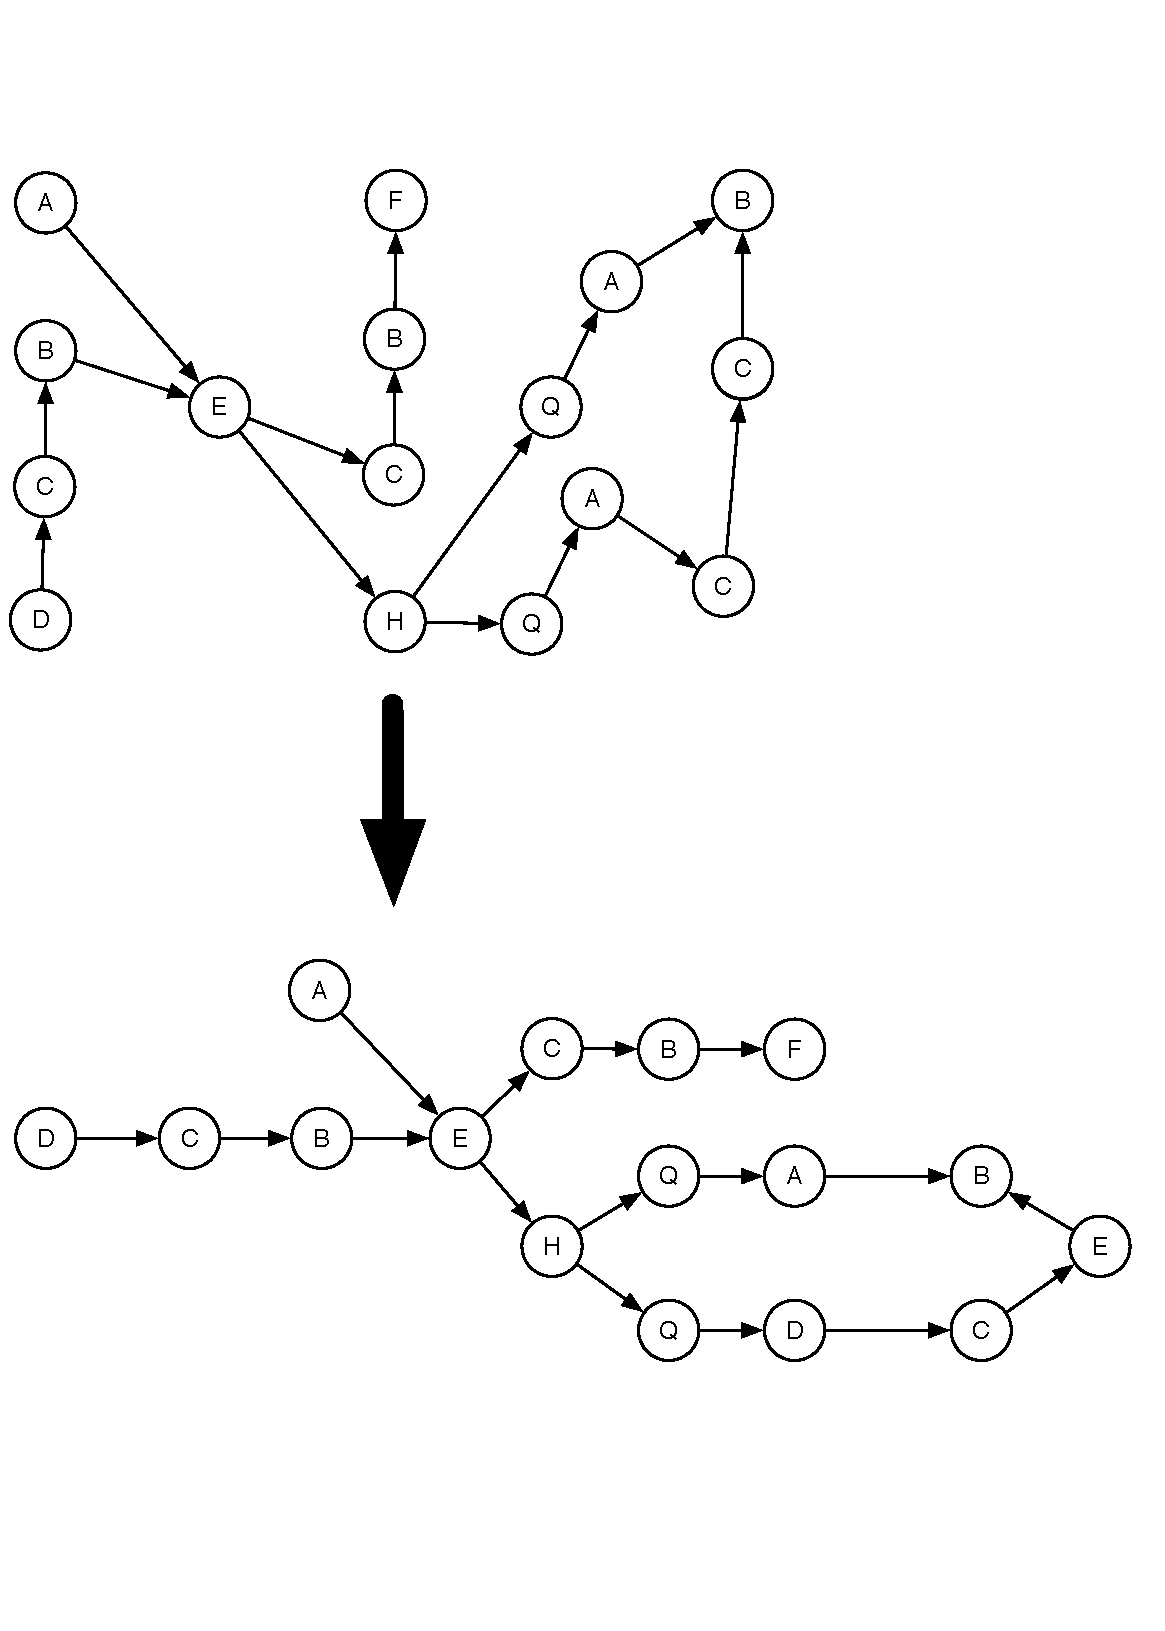
\includegraphics[width=5cm]{images/linearizing}
		\caption{linearizing.}
		\label{fig:linearizing}
	\end{center}
\end{figure}
